\newcommand{\byr}{Br}

\section{Определение экономической эффективности разработки программного обеспечения}

\subsection{Расчёт экономической эффективности использования разработки веб-приложения для продажи квартир}


\FPeval{\totalProgramSize}{10100}
\FPeval{\totalProgramSizeCorrected}{8140}

\FPeval{\normativeManDays}{240} %Tn

\FPeval{\additionalComplexity}{0.20} %Ksl
\FPeval{\complexityFactor}{clip(1 + \additionalComplexity)}

\FPeval{\stdModuleUsageFactor}{0.9} %Kt
\FPeval{\originalityFactor}{0.7} %Kn

\FPeval{\adjustedManDaysExact}{clip( \normativeManDays * \complexityFactor * \stdModuleUsageFactor * \originalityFactor )}
\FPround{\adjustedManDays}{\adjustedManDaysExact}{0}

\FPeval{\daysInYear}{366}
\FPeval{\redLettersDaysInYear}{6}
\FPeval{\weekendDaysInYear}{105}
\FPeval{\vocationDaysInYear}{24}
\FPeval{\workingDaysInYear}{ clip( \daysInYear - \redLettersDaysInYear - \weekendDaysInYear - \vocationDaysInYear ) }

\FPeval{\developmentTimeMonths}{6}
\FPeval{\developmentTimeYearsExact}{clip(\developmentTimeMonths / 12)}
\FPround{\developmentTimeYears}{\developmentTimeYearsExact}{2}
\FPeval{\requiredNumberOfProgrammersExact}{ clip( \adjustedManDays / (\developmentTimeYears * \workingDaysInYear) + 0.5 ) }

% тут должно получаться 2 ))
\FPtrunc{\requiredNumberOfProgrammers}{\requiredNumberOfProgrammersExact}{0}

\FPeval{\tariffRateFirst}{298000} %Tm1
\FPeval{\tariffFactorFst}{3.04}
\FPeval{\tariffFactorSnd}{3.48}


\FPeval{\employmentFstExact}{clip( \adjustedManDays / \requiredNumberOfProgrammers )}
\FPtrunc{\employmentFst}{\employmentFstExact}{0}

\FPeval{\employmentSnd}{clip(\adjustedManDays - \employmentFst)}


\FPeval{\workingHoursInMonth}{160} %Fr
\FPeval{\salaryPerHourFstExact}{clip( \tariffRateFirst * \tariffFactorFst / \workingHoursInMonth )}
\FPeval{\salaryPerHourSndExact}{clip( \tariffRateFirst * \tariffFactorSnd / \workingHoursInMonth )}
\FPround{\salaryPerHourFst}{\salaryPerHourFstExact}{0}
\FPround{\salaryPerHourSnd}{\salaryPerHourSndExact}{0}

\FPeval{\bonusRate}{1.5}
\FPeval{\workingHoursInDay}{8}
\FPeval{\totalSalaryExact}{clip( \bonusRate * 1.4 * 8 * \adjustedManDays)}
\FPround{\totalSalary}{\totalSalaryExact}{0}

\FPeval{\additionalSalaryNormative}{20}

\FPeval{\additionalSalaryExact}{clip( \totalSalary * \additionalSalaryNormative / 100 )}
\FPround{\additionalSalary}{\additionalSalaryExact}{0}

\FPeval{\socialNeedsNormative}{0.5}
\FPeval{\socialProtectionNormative}{34.5}
\FPeval{\socialProtectionFund}{ clip(\socialNeedsNormative + \socialProtectionNormative) }

\FPeval{\socialProtectionCostExact}{clip( (\totalSalary + \additionalSalary) * \socialProtectionFund / 100 )}
\FPround{\socialProtectionCost}{\socialProtectionCostExact}{0}

\FPeval{\stuffNormative}{3}
\FPeval{\stuffCostExact}{clip( \totalSalary * \stuffNormative / 100 )}
\FPround{\stuffCost}{\stuffCostExact}{0}

\FPeval{\timeToDebugCodeNormative}{15}
%\FPeval{\reducingTimeToDebugFactor}{0.3} %?
\FPeval{\adjustedTimeToDebugCodeNormative}{\timeToDebugCodeNormative}

\FPeval{\oneHourMachineTimeCost}{2400}

\FPeval{\machineTimeCostExact}{ clip( \oneHourMachineTimeCost * \totalProgramSizeCorrected / 100 * \adjustedTimeToDebugCodeNormative ) }
\FPround{\machineTimeCost}{\machineTimeCostExact}{0}

\FPeval{\businessTripNormative}{15}
\FPeval{\businessTripCostExact}{ clip( \totalSalary * \businessTripNormative / 100 ) }
\FPround{\businessTripCost}{\businessTripCostExact}{0}

\FPeval{\otherCostNormative}{20}
\FPeval{\otherCostExact}{clip( \totalSalary * \otherCostNormative / 100 )}
\FPround{\otherCost}{\otherCostExact}{0}

\FPeval{\overheadCostNormative}{100}
\FPeval{\overallCostExact}{clip( \totalSalary * \overheadCostNormative / 100 )}
\FPround{\overheadCost}{\overallCostExact}{0}

\FPeval{\overallCost}{clip( \totalSalary + \additionalSalary + \socialProtectionCost + \stuffCost + \machineTimeCost + \businessTripCost + \otherCost + \overheadCost ) }

\FPeval{\supportNormative}{30}
\FPeval{\softwareSupportCostExact}{clip( \overallCost * \supportNormative / 100 )}
\FPround{\softwareSupportCost}{\softwareSupportCostExact}{0}


\FPeval{\baseCost}{ clip( \overallCost + \softwareSupportCost ) }

\FPeval{\profitability}{35}
\FPeval{\incomeExact}{clip( \baseCost / 100 * \profitability )}
\FPround{\income}{\incomeExact}{0}

\FPeval{\estimatedPrice}{clip( \income + \baseCost )}

\FPeval{\localRepubTaxNormative}{3.9}
\FPeval{\localRepubTaxExact}{clip( \estimatedPrice * \localRepubTaxNormative / (100 - \localRepubTaxNormative) )}
\FPround{\localRepubTax}{\localRepubTaxExact}{0}
%\FPeval{\localRepubTax}{0}

\FPeval{\ndsNormative}{20}
\FPeval{\ndsExact}{clip( (\estimatedPrice + \localRepubTax) / 100 * \ndsNormative )}
\FPround{\nds}{\ndsExact}{0}


\FPeval{\sellingPrice}{clip( \estimatedPrice + \localRepubTax + \nds )}

\FPeval{\taxForIncome}{18}
\FPeval{\incomeWithTaxesExact}{clip(\income * (1 - \taxForIncome / 100))}
\FPround{\incomeWithTaxes}{\incomeWithTaxesExact}{0}

\FPeval{\fondSocZ}{clip((\totalSalary + \additionalSalary) * 34 / 100)}

\FPeval{\fondEN}{clip((\totalSalary + \additionalSalary) * 4 / 100)}

\FPeval{\fondTimeMachine}{clip(\totalProgramSizeCorrected * 3 * 0.55 / 100)}

\FPeval{\prochieZatraty}{clip(\totalSalary * 20 / 100)}

\FPeval{\zatrariPoStatie}{clip(2900 * 20 / 100)}

\FPeval{\polnaySebes}{clip(2900 + \zatrariPoStatie)}

\FPeval{\planovayPrib}{clip(1022* (1-18/100))}

\FPeval{\progCena}{clip(1022 + \polnaySebes)}

\FPeval{\NDS}{clip(\progCena * 20 / 100)}

\FPeval{\progCenaNDS}{clip(\progCena + \NDS)}

\FPeval{\Ko}{clip(\progCenaNDS * 30 / 100)}

\FPeval{\progCenaNDSKO}{clip(\progCenaNDS + \Ko)}

\FPeval{\zEconomia}{clip(1.5 * 1* 3860 * (1+ 20 / 100) * (1+ 34/100) )}


% End Calculations
Расчёт объёма ПО.  Для расчёта плановой сметы затрат на разработку ПО необходимо определить объём ПО.
Общий объём программного продукта определяется исходя из количества и объёма функций, реализуемых программой:
\begin{equation}
\label{eq:econ:total_program_size}
V_{o} = \sum_{i = 1}^{n} V_{i} \text{\,,}
\end{equation}
\begin{explanation}
	где & $ V_{i} $ & объём отдельной функции ПО, LoC; \\
	& $ n $ & общее число функций.
\end{explanation}

Тогда по формуле получаем: 
\begin{equation}
\label{eq:econ:complexity_coeff_calc}
\text V_{\text{o}} = \SI{\totalProgramSize}{\text{LoC}}.
\end{equation}

В связи с использованием более совершенных средств  автоматизации 
уточнённый объём составил:
\begin{equation}
\label{eq:econ:complexity_coeff_calc}
\text V_{\text{y}} = \SI{\totalProgramSizeCorrected}{\text{LoC}}.
\end{equation}

\begin{table}[ht]
	\caption{Перечень и объём функций программного продукта}
	\label{table:econ:function_sizes}
	\centering
	\begin{tabular}{| >{\centering}m{0.12\textwidth}
			| >{\raggedright}m{0.40\textwidth}
			| >{\centering}m{0.18\textwidth}
			| >{\centering\arraybackslash}m{0.18\textwidth}|}
		
		\hline
		\multirow{2}{0.12\textwidth}[-0.5em]{\centering \No{}}
		& \multirow{2}{0.40\textwidth}[-0.55em]{\centering Наименование (содержание)}
		& \multicolumn{2}{c|}{\centering Объём функции, LoC} \tabularnewline
		
		\cline{3-4} &
		& { по каталогу}
		& { уточненный} \tabularnewline
		
		\hline
		1 & Организация ввода информации & \num{160} & \num{140} \tabularnewline
		\hline
		2 & Формирование базы данных 	& \num{2180} & \num{1950} \tabularnewline
		\hline
		3 & Организация поиска и поиск в базе данных  & \num{5490} & \num{3950} \tabularnewline
		\hline
		4 & Обработка файлов  & \num{730} & \num{690} \tabularnewline
		\hline
		5 & Формирование файла в  & \num{1030} & \num{940} \tabularnewline
		\hline
		6 & Графический вывод результатов & \num{510} & \num{470} \tabularnewline
		\hline
		Итог & & {\num{\totalProgramSize}} & {\num{\totalProgramSizeCorrected}} \tabularnewline
		
		\hline
		
	\end{tabular}
\end{table}

Общая трудоёмкость небольших проектов рассчитывается по формуле:
\begin{equation}
\label{eq:econ:effort_common}
\text{Т}_\text{о} = \text{Т}_\text{н} \cdot
\text{К}_\text{с} \cdot
\text{К}_\text{т} \cdot
\text{К}_\text{н} \text{\,,}
\end{equation}
\begin{explanation}
	где & $ \text{К}_\text{с} $ & коэффициент, учитывающий сложность ПО, $ \text{К}_{\text{с}} = \num{\complexityFactor}$; \\
	& $ \text{К}_\text{т} $ & поправочный коэффициент, учитывающий степень использования при разработке стандартных модулей,
	$ \text{К}_{\text{т}} = \num{\stdModuleUsageFactor}$;\\
	& $ \text{К}_\text{н} $ & коэффициент, учитывающий степень новизны ПО, $ \text{К}_\text{н} = \num{\originalityFactor}$.
\end{explanation}

Таким образом:
\begin{equation}
\label{eq:econ:effort_common_calc}
\text{Т}_\text{о} = \num{\normativeManDays} \cdot \num{\complexityFactor} \cdot \num{\stdModuleUsageFactor} \cdot \num{\originalityFactor} \approx \SI{\adjustedManDays}{\text{чел.}/\text{дн.}}
\end{equation}

Рассчитаем число исполнителей проекта по формуле:
\begin{equation}
\label{eq:econ:num_of_programmers}
\text{Ч}_\text{р} = \frac{\text{Т}_\text{о}}{\text{Т}_\text{р} \cdot \text{Ф}_\text{эф}} \text{\,,}
\end{equation}
\begin{explanation}
	где & $ \text{Т}_\text{о} $ & общая трудоемкость разработки проекта, $ \text{Т}_\text{о} = \num{\adjustedManDays}$ 
	$ \text{чел.}/\text{дн.} $; \\
	& $ \text{Ф}_\text{эф} $ & эффективный фонд времени работы одного работника в течение года, $ \text{Ф}_\text{эф} = \num{\workingDaysInYear} $ дн.; \\
	& $ \text{Т}_\text{р} $ & срок разработки проекта,$ \text{Т}_\text{р} = \num{\developmentTimeYears} $  лет.
\end{explanation}

Таким образом:
\begin{equation}
\label{eq:econ:num_of_programmers_calc}
\text{Ч}_\text{р} =
\frac{\num{\adjustedManDays}}
{\num{\developmentTimeYears} \cdot \num{\workingDaysInYear}}
\approx \SI{\requiredNumberOfProgrammers}{\text{рабочих}}.
\AfterEndEnvironment{equation}{\vspace{0pt}}
\end{equation}

Затраты на разработку ПО включают:
\begin{itemize}
	\item  затраты на основную заработную плату разработчиков; 
	\item  затраты на дополнительную заработную плату разработчиков; 
	\item  отчисления на социальные нужды; 
	\item  затраты по статье Машинное время; 
	\item  затраты на сопровождение и адаптацию ПО; 
	\item  прочие затраты;
\end{itemize}

Основная заработная плата  разработчиков  программного  средства рассчитывается по формуле:
\begin{equation}
\label{eq:econ:total_salary}
\text{З}_{\text{о}} = 
\text{К}_{\text{пр}} \cdot 
\sum^{n}_{i = 1}
\text{Т}_{\text{ч}}^{i} \cdot
\text{Т}_{\text{ч}} \cdot
\text{Ф}_{\text{эi}}
\text{\,,}
\end{equation}
\begin{explanation}
	где & $ \text{Т}_{\text{ч}}^{i} $ & часовая тарифная ставка \mbox{$ i $-го} исполнителя, 
	$ \text{Т}_{\text{ч}}^{i} = \num{1,4}$; \\
	& $ \text{Т}_{\text{ч}} $ & количество часов работы в день, $ \text{Т}_{\text{ч}}= \num{8}$; \\
	& $ \text{Ф}_{\text{эi}} $ & плановый фонд рабочего времени \mbox{$ i $-го} исполнителя,
	$ \text{Ф}_{\text{эi}} = \SI{\adjustedManDays} $; \\
	& $ \text{К}_{\text{пр}} $ & коэффициент премий, установленный за выполнение  плановых показателей,
	$ \text{К}_{\text{пр}} = \num{\bonusRate}$.
\end{explanation}

Тарифная  ставка 1-го  разряда с января 2017 года составляет 31 рубль. Предприятия имеют право увеличивать  тарифную  ставку,  но  не  более  чем минимальная заработная плата (в настоящее время 265 руб.).  В  нашей компании месячная тарифная ставка 1-го разряда равна 100 руб.  

Таким образом:
\begin{equation}
\label{eq:econ:total_salary_calc}
\text{З}_{\text{о}} = \num{\bonusRate} \cdot \num{1,4} \cdot \num{8} \cdot  \SI{\adjustedManDays} = \SI{\totalSalary}{\text{руб}}.
\end{equation}

\begin{table}[ht]
	\caption{ Разряды, ставки и тарифные коэффициенты работников}
	\label{table:econ:programmers}
	\begin{tabular}{
			| >{\centering}m{0.2\textwidth}
			| >{\centering}m{0.15\textwidth}
			| >{\centering}m{0.18\textwidth}
			| >{\centering}m{0.18\textwidth}
			| >{\centering\arraybackslash}m{0.15\textwidth}|
		}
		\hline
		Наименование должности & Разряд & Тарифный коэффициент & Месячная тарифная ставка&Часовая тарифная ставка, руб. \\
		\hline
		Ведущий программист & $ \num{10} $ & $ \num{2,48} $ & $ \num{248} $ & $ \num{1,4} $\\
		\hline
	\end{tabular}
\end{table}

Дополнительная заработная плата  определяется по следующей формуле: 
\begin{equation}
\label{eq:econ:additional_salary}
\text{З}_{\text{д}} =
\frac {\text{З}_{\text{о}} \cdot \text{Н}_{\text{д}}}
{100} \text{\,,}
\end{equation}
\begin{explanation}
	где & $ \text{Н}_{\text{д}} $ & норматив дополнительной заработной платы, $ \num{20} \% $.
\end{explanation}
\begin{equation}
\label{eq:econ:additional_salary_calc}
\text{З}_{\text{д}} =
\frac{\num{\totalSalary} \cdot 20}
{100} \approx 
%\SI{\additionalSalary}{\text{руб}} \text{\,.}
\SI{\additionalSalary}{\text{руб}}.
\AfterEndEnvironment{equation}{\vspace{0pt}}
\end{equation}

Отчисления в Фонд социальной защиты  населения  определяются  в соответствии с действующими законодательными актами по нормативу в процентном соотношении к фонду основной и дополнительной зарплаты исполнителей, определённой по нормативу, установленному в целом по организации:
\begin{equation}
\label{eq:econ:additional_salary1}
\text{Р}_{\text{соц}} = \frac{(\text{З}_{\text{о}} + \text{З}_{\text{д}}) \cdot \text{Н}_{\text{соц}}}{\num{100}} \text{\,,}
\end{equation}
\begin{explanation}
	где & $ \text{Н}_{\text{соц}} $ &ставка отчислений в Фонд социальной защиты населения, установленная законодательством,, $ \num{34} \% $.
\end{explanation}

Таким образом:
\begin{equation}
\label{eq:econ:additional_salary2}
\text{Р}_{\text{соц}} = \frac{(\SI{\totalSalary} +  \SI{\additionalSalary}) \cdot \num{34}}{\num{100}} = 
%\SI{\fondSocZ}\text{руб.}
\SI{\fondSocZ}{\text{руб}}.
\end{equation}

Затраты по статье «Единый налог от фонда оплаты труда». В эту статью включаются отчисления в Фонд содействия занятости, чрезвычайный налог, которые определяются по следующей формуле: 
\begin{equation}
\label{eq:econ:additional_salary3}
\text{Р}_{\text{ен}} = \frac{(\text{З}_{\text{о}} + \text{З}_{\text{д}}) \cdot \text{Н}_{\text{ен}}}{\num{100}} \text{\,,}
\end{equation}
\begin{explanation}
	где & $ \text{Н}_{\text{ен}} $ & ставка единого налога, установленного законодательством, $ \num{4} \% $.
\end{explanation}
\begin{equation}
\label{eq:econ:additional_salary4}
\text{Р}_{\text{соц}} = \frac{(\SI{\totalSalary} +  \SI{\additionalSalary}) \cdot \num{4}}{\num{100}} = 
\SI{\fondEN}{\text{руб}}.
\end{equation}

Затраты по статье «Машинное время»  (Рм)  включают  оплату машинного времени, необходимого для разработки и  отладки  ПО.  Они 
определяются в машино-часах по нормативам на 100 LOC в  зависимости от характера решаемых задач и типа компьютера. 

Рассчитываются по формуле:
\begin{equation}
\label{eq:econ:additional_salary5}
\text{Р}_{\text{ен}} = \frac{\text{Ц}_{\text{м}} \cdot \text{V}_{\text{o}} \cdot \text{Н}_{\text{мз}}}{\num{100}} \text{\,,}
\end{equation}
\begin{explanation}
	где & $ \text{Н}_{\text{мз}} $ &  норматив  расхода  машинного  времени  на  отладку  100 LOC, $ \num{3} \% $;\\
	& $ \text{Ц}_{\text{м}} $ & цена одного машино-часа, 0,55 руб;\\
	& $ \text{V}_{\text{o}} $ & общий объём, $ \SI{\totalProgramSizeCorrected}{\text{LOC}}$;.
\end{explanation}

\begin{equation}
\label{eq:econ:additional_salary6}
\text{Р}_{\text{ен}} = \frac{\num{0,55} \cdot \SI{\totalProgramSizeCorrected} \cdot \text{ } \num{3}}{\num{100}} = 
\SI{\fondTimeMachine}{\text{руб}}.
\AfterEndEnvironment{equation}{\vspace{0pt}}
\end{equation}

Прочие затраты  включают  затраты  на  приобретение  и  подготовку 
специальной научно-технической информации и специальной литературы. 

Рассчитываются по формуле: 
\begin{equation}
\label{eq:econ:additional_salary7}
\text{П}_{\text{з}} = \frac{\text{З}_{\text{о}} \cdot \text{Н}_{\text{пз}}}{\num{100}} \text{\,,}
\end{equation}
\begin{explanation}
	где & $ \text{Н}_{\text{пз}} $ & норматив прочих затрат, $ \num{20} \% $;\\
	& $ \text{З}_{\text{о}} $ & сумма основной заработной платы.
\end{explanation}

Рассчитаем прочие затраты:
\begin{equation}
\label{eq:econ:additional_salary8}
\text{П}_{\text{з}} = \frac{ \SI{\totalSalary} \cdot \num{20}}{\num{100}} =
\SI{\prochieZatraty}{\text{руб}}.
\end{equation}

Организация-разработчик  осуществляет сопровождение ПО, соответственно несёт затраты, на которые составляется смета, оплачиваемая заказчиком по договору. Затраты  по статье  «Сопровождение  и адаптация  ПО» определяются по нормативу  по формуле: 

\begin{equation}
\label{eq:econ:additional_salary9}
\text{П}_{\text{з}} = \frac{\text{C}_{\text{пр}} \cdot \text{Н}_{\text{с}}}{\num{100}} \text{\,,}
\end{equation}
\begin{explanation}
	где & $ \text{С}_{\text{пр}} $ & общая сумма производственной себестоимости, $ \num{2900} $ руб;\\
	& $ \text{Н}_{\text{с}} $ &  норматив расходов на сопровождение и адаптацию, $ \num{20} \% $.
\end{explanation}

Итого:
\begin{equation}
\label{eq:econ:additional_salary10}
\text{Р}_{\text{с}} = \frac{ \num{2900} \cdot \num{20}}{\num{100}} = 
\SI{\zatrariPoStatie}{\text{руб}}.
\AfterEndEnvironment{equation}{\vspace{0pt}}
\end{equation}

Полная себестоимость ПО:

\begin{equation}
\label{eq:econ:additional_salary11}
\text{C}_{\text{п}} = \text{C}_{\text{пр}} + \text{Р}_{\text{с}} \text{\,,}
\AfterEndEnvironment{equation}{\vspace{-30pt}}
\end{equation}

\begin{equation}
\label{eq:econ:additional_salary12}
\text{С}_{\text{п}} = \num{2900} + \SI{\zatrariPoStatie} =
\SI{\polnaySebes}{\text{руб}}.
\AfterEndEnvironment{equation}{\vspace{20pt}}
\end{equation}

При разработке программного обеспечения по индивидуальному заказу экономический эффект рассчитывается для организации-разработчика. Необходимо  также  описать и возможный эффект от  использования программного продукта, который получит пользователь. 

Критерием  интегрированной  экономической эффективности у разработчика выступает чистая прибыль, остающаяся в распоряжении 
предприятия от реализации программного средства, а у пользователя этим критерием служит экономия трудовых, материальных и финансовых ресурсов.

Прибыль от реализации ПО за вычетом налога на прибыль является чистой прибылью ($ \text{П}_{\text{Ч}} $),  остаётся  организации-разработчику  и  представляет собой экономический эффект от создания нового программного продукта:

\begin{equation}
\label{eq:econ:additional_salary13}
\text{П}_{\text{Ч}} = { \text{П}_{\sum} \cdot (\text{1} - \text{Н}_{\text{П}} / \num{100}) } \text{\,,}
\end{equation}
\begin{explanation}
	где & $ \text{П}_{\sum} $ & плановая прибыль от реализации  ПО,  принимаем $ \text{П}_{\sum} = \num{1022} $ руб;\\
	& $ \text{Н}_{\text{с}} $ &  ставка налога на прибыль, $\text{Н}_{\text{с}} = \num{18} \% $.
\end{explanation}

\begin{equation}
\label{eq:econ:additional_salary14}
\text{П}_{\text{Ч}}^{\text{1,2,3,4}} = { \num{1022} \cdot (\text{1} - \num{18} / \num{100}) } = 
{\SI{\planovayPrib}{\text{руб}}.}
\end{equation}

Прогнозируемая цена ПО без налогов определяется по формуле:

\begin{equation}
\label{eq:econ:additional_salary15}
\text{Ц}_{\text{п}} = { \text{П}_{\sum} + \text{C}_{\text{п}}} \text{\,,}
\end{equation}
\begin{explanation}
	где & $ \text{П}_{\sum} $ & плановая прибыль от реализации  ПО,  принимаем $ \text{П}_{\sum} = \num{1022} $ руб;\\
	& $ \text{С}_{\text{п}} $ & полная себестоимость ПО,ь, $\text{С}_{\text{п}} = \SI{\polnaySebes} $.
\end{explanation}

Итого:
\begin{equation}
\label{eq:econ:additional_salary16}
\text{Ц}_{\text{п}} = { \SI{\polnaySebes} + \num{1022}} =
{\SI{\progCena}{\text{руб}}.}
\end{equation}

Отпускная цена (цена реализации) ПО включает налог на добавленную стоимость:
\begin{equation}
\label{eq:econ:additional_salary17}
\text{Ц}_{\text{о}} = { \text{Ц}_{\text{п}} + \text{НДС}} \text{\,,}
\end{equation}
\begin{explanation}
где & $ \text{НДС} $ &  налог на добавленную стоимость, $ \text{НДС} = \SI{\NDS} (20 \text{\% от } \text{Ц}_{\text{п}}) $ руб
\end{explanation}

\begin{equation}
\label{eq:econ:additional_salary18}
\text{Ц}_{\text{о}} = \SI{\progCena} + \SI{\NDS} \text{ } = \text{ } {\SI{\progCenaNDS}{\text{руб}}.}
\end{equation}

Для определения  интегрированного  экономического эффекта от использования нового ПО у  потребителя необходимо  сравнить  расходы по всем основным статьям сметы затрат на эксплуатацию нового ПО (расходы на заработную плату с начислениями,  затраты на  расходные  материалы, расходы на машинное  время) с расходами  по  соответствующим  статьям базового варианта. При этом за базовый вариант принимаем ручной вариант, так как  автоматизация отсутствует. Создание нового ПО окажется экономически целесообразным лишь в том случае, если все капитальные затраты окупятся  за  счёт  получаемой  экономии  в  ближайшее  время  (до  2 лет). 

Общие капитальные вложения ($ \text{К}_{\text{в}} $)  потребителя, связанные с приобретением, внедрением и использованием ПО, рассчитываются по 
формуле: 
\begin{equation}
\label{eq:econ:additional_salary19}
\text{К}_{\text{в}} = { \text{Ц}_{\text{о}} + \text{К}_{\text{о}}} \text{\,,}
\end{equation}
\begin{explanation}
	где & $ \text{Ц}_{\text{о}} $ &  затраты пользователя  на приобретение ПО  по  отпускной  цене у 
	разработчика с учётом стоимости услуг по эксплуатации и сопровождению, $ \text{Ц}_{\text{о}} = \SI{\progCenaNDS} {\text{руб}} $;\\ 
	& $ \text{К}_{\text{о}} $ &  затраты пользователя на освоение программного обеспечения, $ \text{К}_{\text{о}} = \SI{\Ko} {\text{ руб }} (30 \text{\% от } \text{Ц}_{\text{о}}) $
\end{explanation}

\begin{equation}
\label{eq:econ:additional_salary20}
\text{К}_{\text{в}} = \SI{\progCenaNDS} + \SI{\Ko} {\text{ }} = {\text{ }} {\SI{\progCenaNDSKO}{\text{руб}}.}
\end{equation}

Внедрение нового ПО позволит пользователю сэкономить на заработной плате в связи с  высвобождением  работника,  т.е.  практически получить на эту сумму  дополнительную прибыль.  Прирост  прибыли  в данном случае определяется по формуле:
\begin{equation}
\label{eq:econ:total_salary21}
\text{З}_{\text{о}} = 
\text{К}_{\text{пр}} \cdot 
\sum^{n}_{i = 1}
\text{Ч} \cdot
\text{З}_{\text{i}} \cdot
(1+ 
\frac{\text{Н}_{\text{Д}}}{\num{100}}
) \cdot
(1+ 
\frac{\text{Н}_{\text{соц}}}{\num{100}}
)
\text{\,,}
\end{equation}
\begin{explanation}
	где & $ \text{К}_{\text{пр}} $ &   коэффициент премий, $ \text{К}_{\text{пр}} = \num{1,5} $;\\ 
	& $ \text{Ч} $ &  абсолютное высвобождение работников, $ \text{Ч} = \num{1} $;\\
	& $ \text{З}_{\text{i}} $ & годовая заработная плата высвобождаемых работников, $ \text{З}_{\text{i}} = \num{3860} $;\\
	& $ \text{Н}_{\text{Д}} $ & норматив дополнительной заработной платы, $ \text{Н}_{\text{Д}} = \num{20} {\text{\%}}$;\\
	& $ \text{Н}_{\text{соц}} $ & ставка отчислений в Фонд социальной защиты населения, $ \text{Н}_{\text{соц}} = \num{34} {\text{\%}}$.
\end{explanation}

\begin{equation}
\label{eq:econ:total_salary22}
\text{З}_{\text{о}} = 
\num{1,5} \cdot 
\num{1} \cdot 
\num{3860} \cdot 
(1+ 
\frac{\num{20}}{\num{100}}
) \cdot
(1+ 
\frac{\num{34}}{\num{100}}
) =
{\SI{\zEconomia}{\text{руб}}.}
\end{equation}

Экономия заработной платы  выступает  в  качестве  экономического эффекта, то есть  чистой  прибыли, которая остается в распоряжении предприятия: $ \text{К}_{\text{пр}} = {\SI{\zEconomia}{\text{руб}}.} $

Полученные суммы  результата (чистой прибыли) и затрат (капительных вложений) по годам необходимо привести к единому моменту 
времени – расчётному году (2017) путём умножения результатов и затрат на коэффициент дисконтирования αt, который рассчитывается по формуле:
\begin{equation}
\label{eq:econ:total_salary23}
\alpha_{\text{t}} = 
\frac{\num{1}}{(1 + E_{\text{н}})^{t-t_{p}}}
\text{\,,}
\end{equation}
\begin{explanation}
	где & $ \text{E}_{\text{н}} $ &   коэффициент премий, $ \text{E}_{\text{н}} = \num{15} \% $;\\ 
	& $ \text{t} $ &   порядковый номер расчётного года, $ \text{t} = \num{1} $;\\
	& $ \text{t}_{\text{p}} $ &  порядковый номер года, затраты и результаты  которого  приводятся  к 
	расчётному году.
\end{explanation}

Рассчитаем коэффициенты дисконтирования:
\begin{equation}
\label{eq:econ:total_salary24}
\alpha_{\text{1}} = 
\frac{\num{1}}{(1 + 0,15)^{1-1}} = 
\text{\,1,}
\end{equation}

\begin{equation}
\label{eq:econ:total_salary25}
\alpha_{\text{2}} = 
\frac{\num{1}}{(1 + 0,15)^{2-1}} = 
\text{\,0,87,}
\end{equation}

\begin{equation}
\label{eq:econ:total_salary26}
\alpha_{\text{3}} = 
\frac{\num{1}}{(1 + 0,15)^{3-1}} = 
\text{\,0,76,}
\end{equation}

\begin{equation}
\label{eq:econ:total_salary27}
\alpha_{\text{4}} = 
\frac{\num{1}}{(1 + 0,15)^{4-1}} = 
\text{\,0,66}
\end{equation}

Расчёт  интегрированного  экономического эффекта у пользователя осуществляется по формуле:
\begin{equation}
\label{eq:econ:total_salary28}
\text{Э}_{\text{инт}} = 
\sum^{n}_{t = 1}
\text{ЧДД} = 
\sum^{n}_{t = 1}
(\text{P}_{t} \cdot \alpha_{\text{t}} - \text{З}_{t} \cdot \alpha_{\text{t}})
\text{\,,}
\end{equation}
\begin{explanation}
	где & $ \text{т} $ &  расчётный период, n = 4 года;\\ 
	& $ \text{P}_{\text{t}} $ &  чистый доход, полученный в году t, руб;\\
	& $ \text{З}_{\text{t}} $ &  затраты (инвестиции) в году t, руб.;\\
	& $ \alpha_{\text{t}} $ &  коэффициент дисконтирования.\\
	%& $ \alpha_{\text{t}} $  коэффициент дисконтирования.
\end{explanation}

ЧДД это чистый  дисконтированный  доход  (превышение суммарных денежных поступлений над суммарными затратами с учётом неравномерности  эффектов, относящихся к различным моментам времени).

Расчёт  интегрированного  экономического эффекта за весь период использования ПО (4  года)  представлен в  таблице ниже.

\begin{longtable}[l]{| >{\raggedright}m{0.2\textwidth}
		| >{\centering}m{0.09\textwidth}
		| >{\centering}m{0.12\textwidth}
		| >{\centering}m{0.09\textwidth}
		| >{\centering}m{0.1\textwidth}
		| >{\centering}m{0.1\textwidth}
		| >{\centering\arraybackslash}m{0.11\textwidth}
		|}
	\caption{ Расчёт интегрированного экономического эффекта }
	\label{table:econ:calculation_cost_and_price}
	
	\hline
	{\begin{center}Наименование\end{center} } & Ед. измер & Усл. обозн. & 2018 & 2019 & 2020 & 2021\\

	\hline
	Чистая прибыль & руб & $\text{П}_{\text{Ч}} $ & 0 & 9310,32 & 9310,32 & 9310,32 \\
	\hline
	
	Результат с учётом фактор времени  & руб & $\text{P}_{t} \cdot \alpha_{\text{t}}$ & 0 & 8099,98 & 7075,84 & 6144,81 \\
	\hline
	
	Капитальные вложения   & руб & $\text{К}_{в} $ & 6842 & 0 & 0 & 0 \\
	\hline
	
	Затраты : & & & & & & \\
	\hline 
	
	Результат с учётом фактор времени  & руб & $\text{З}_{t} \cdot \alpha_{\text{t}}$ & 6842 & 0 & 0 & 0 \\
	\hline
	
	Чистый дисконтированный доход & руб & ЧДД & - 6842 & 8099,98 & 7075,84 & 6144,81 \\
	\hline
	
	Чистый дисконтированный доход с нарастающим итогом & руб & $\text{Э}_{\text{инт}} $ & - 6842 & 1257,98 & 8333,82 & 14478,63 \\
	
	\hline
	
	Коэффициент дисконтирования &  & $\alpha_{\text{t}}$ & 1 & 0,87 & 0,76 & 0,66 \\
	\hline
	
\end{longtable}

\begin{equation}
\label{eq:econ:total_salary29}
\text{Э}_{\text{инт}} = 14478,63 \text{ руб.}
\end{equation}

Чистый дисконтированный доход имеет максимальное значение во втором году в реализации проекта и составляет  8099,98 руб., а 
интегрированный экономический эффект имеет положительное значение и за четыре года реализации проекта составит 14478,63 руб. 
На рисунках ниже представлены диаграммы  чистого дисконтированного дохода  и  интегрированного экономического эффекта.

\begin{figure}[!htb]
	\centering
	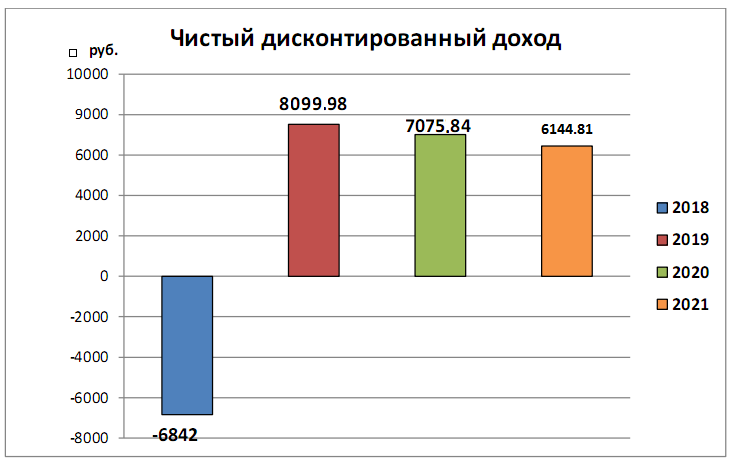
\includegraphics[scale=0.7]{economica_ris1.png}
	\caption{ Гистограмма чистого дисконтированного дохода}
	\label{fig:sec_usage::signIn}
\end{figure}

\begin{figure}[!htb]
	\centering
	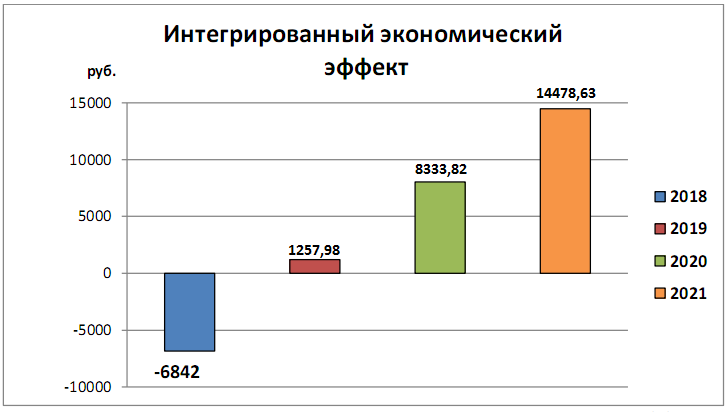
\includegraphics[scale=0.7]{economica_ris2.png}
	\caption{ Гистограмма интегрированного экономического эффекта }
	\label{fig:sec_usage::signIn}
\end{figure}

Расчёт срока окупаемости затрат.  Срок окупаемости  –  это количество лет, в течение которых  затраченные средства возвратятся в виде чистого дохода. Иначе, это период времени, который необходим для возмещения  затрат    за счёт дохода.  Срок  окупаемости $\text{Т}_{\text{ок}} $ из неравенства: 

\begin{equation}
\label{eq:econ:total_salary31}
\text{Т}_{\text{ок}} = 
\sum^{n}_{t = 1}
\text{P}_{t} \cdot \alpha_{\text{t}} \ge 
\sum^{n}_{t = 1}
\text{С}_{t} \cdot \alpha_{\text{t}}
\text{\,,}
\end{equation}

Если подставить в неравенство значения за 4 года, то получим следующую ситуацию:
\begin{equation}
\label{eq:econ:total_salary30}
\text{Т}_{\text{ок}} = 
\num{21320,63} \ge
\num{7969,2} 
\end{equation}

Неравенство выполняется, из чего следует что срок окупаемости равен: $ Т\text{Т}_{\text{ок}} = \text{ 4 года.} $
 
Расчёт рентабельности  инвестиций.  Рентабельность  инвестиций является одним из основных показателей экономической эффективности использования  нового  ПО.  

Рентабельность  инвестиций  определяется  по 
формуле: 

\begin{equation}
\label{eq:econ:total_salary33}
\text{Р}_{\text{и}} = 
\frac{\sum^{n}_{t = 1} \text{P}_{t} \cdot \alpha_{\text{t}}}{\sum^{n}_{t = 1} \text{З}_{t} \cdot \alpha_{\text{t}}}
\cdot \num{100} \text{ \%}
\text{\,,}
\end{equation}
\begin{explanation}
	где & $ \text{P}_{\text{t}} $ &  чистый доход, полученный в году t, руб;\\
	& $ \text{З}_{\text{t}} $ &  затраты (инвестиции) в году t, руб.;\\
	& $ \alpha_{\text{t}} $ &  коэффициент дисконтирования.\\
	%& $ \alpha_{\text{t}} $  коэффициент дисконтирования.
\end{explanation}

С учётом результатов таблицы 6.3  рентабельность  инвестиций  в 
проект составит:

\begin{equation}
\label{eq:econ:total_salary34}
\text{Р}_{\text{и}} = 
\frac{14478,63}{6842}
\cdot \num{100} \text{ \%} =
\text{211 \%}
\end{equation}

В  процессе  расчёта  показателей экономической эффективности использования разработки  и внедрения  защиты байткода виртуальной машины джава от декомпиляции были получены следующие результаты: 
\begin{itemize}
	\item чистый дисконтированный доход имеет максимальное значение во 
	втором году реализации проекта и составляет $ \text{ЧДД} = \num{8099,98} $;
	\item интегрированный  экономический эффект имеет положительное 
	значение и за четыре года  проекта  реализации  составит   $ \text{Э}_{\text{инт}} = \num{14478,63} $ 
	руб.; 
	\item срок окупаемости затрат  $ \text{Т}_{\text{ок}} = \text{ 4 года} $; 
	\item рентабельность инвестиций $ \text{Р}_{\text{и}} = \text{ 211 \%.} $  
\end{itemize}}

Таким образом, разработка и внедрение веб-приложения для продажи квартир является перспективным для коммерческого 
успеха.
